\subsection{Towards ductile fracture}

\subsectioncover

\begin{frame}{}
The free energy takes the following form
\begin{align}
    \pi(\defgrad, \defgrad^p, \plasticstrain, d, \grad d) = \pi_\elastic(\defgrad, \defgrad^p, d) + \pi_\plastic(\plasticstrain, d) + \pi_\fracture(d, \grad d).
\end{align} \\
The elastic energy is defined as
\begin{subequations}
\begin{align}
    \pi_\elastic(\defgrad, \defgrad^p, d) &= g^e(d) \pi_\elastic^\activeenergy(\defgrad, \defgrad^p) + \pi_\elastic^\inactiveenergy(\defgrad), \\
    \pi_\elastic^\activeenergy(\defgrad, \defgrad^p) &= H(J-1) \left[ \dfrac{1}{2} K_s \left( \dfrac{1}{2} (J^2-1) - \ln{J} \right) \right] + \dfrac{1}{2} \mu_s \left( \overbar{\bs{C}} : {\bs{C}^p}^{-1} - 3 \right), \\
    \pi_\elastic^\inactiveenergy(\defgrad) &= H(1-J) \left[ \dfrac{1}{2} K_s \left( \dfrac{1}{2} (J^2-1) - \ln{J} \right) \right].
\end{align}
\end{subequations} \\
The plastic energy is defined as
\begin{align}
    \pi_\plastic(\plasticstrain) &= g^p(d) \sigma_Y \plasticstrain + g^h(d) \dfrac{1}{2} h \plasticstrain^2.
\end{align}
\begin{exampleblock}{}
    See \texttt{hyperelasticity.pdf} for other hyperelastic potentials with tension-compression asymmetry. \\
    See \texttt{plasticity.pdf} for a detailed derivation.
\end{exampleblock}
\end{frame}

\begin{frame}{}
\vspace{-1em}
Balance laws and constitutive equations:
\begin{align}
    \divergence \bs{P} + \rho_0 \bs{B} &= \bs{0}, \\
    - \divergence \pi_{, \grad d} + \textcolor{dukeroyal}{\pi_{, d}} &\geqslant 0, \quad \dot{d} \geqslant 0, \\
    \rho_0 r - \pi_{, \plasticstrain} \dot{\plasticstrain} - \pi_{, d} \dot{d} &= \rho_0 c \dot{T},
\end{align} \\
The constitutive relation between the Kirchhoff stress and the deformation gradient is
\begin{subequations}
\begin{align}
    & \bs{\tau} = \textcolor{dukeroyal}{g^e(d)}\bs{\tau}^\activeenergy + \bs{\tau}^\inactiveenergy, \\
    & \bs{\tau}^\activeenergy = \dfrac{1}{2} H(J-1) K_s (J^2-1) \bs{I} + \mu_s \dev(\bs{b}^e), \\
    & \bs{\tau}^\inactiveenergy = \dfrac{1}{2} H(1-J) K_s (J^2-1) \bs{I}.
\end{align}
\end{subequations} \\
The Kuhn-Tucker loading/unloading conditions are
\begin{align}
    & \phi(\bs{N}^p, \plasticstrain, d) = \norm{\dev(\bs{\tau})} - \sqrt{\dfrac{2}{3}} \left[ \textcolor{dukeroyal}{g^p(d)} \sigma_Y + \textcolor{dukeroyal}{g^h(d)} h \plasticstrain \right] \leqslant 0, \quad \dot{\plasticstrain} \geqslant 0, \quad \dot{\plasticstrain}\phi(\bs{N}^p, \plasticstrain, d) = 0,
\end{align} \\
and the flow rule is \\
\begin{align}
    & \dot{\defgrad}^p {\defgrad^p}^{-1} = \dot{\plasticstrain} \bs{N}^p, \quad \bs{N}^p = \sqrt{\dfrac{3}{2}} \dfrac{\dev(\bs{\tau})}{\norm{\dev(\bs{\tau})}}, \quad \det(\defgrad^p) = 1.
\end{align}
\end{frame}

\begin{frame}{}
\contenttitle{Unperturbed elastic-plastic behavior} \\
\begin{figure}[htb!]
    \centering
    \begin{subfigure}{0.48\textwidth}
        \centering
        \begin{tikzpicture}
            \begin{axis}[
                cycle list name=color list,
                width=\textwidth,
                height=0.8\textwidth,
                xmin=0,
                ymin=0,
                ymax=600,
                xlabel=$\varepsilon$,ylabel=$\sigma$,
                legend style={at={(0.05,0.95)},anchor=north west},
                legend style={nodes={scale=0.6, transform shape}},
                legend cell align={left},
                every axis plot/.append style={thick}
            ]
                \addplot +[mark=none] table[x expr=\thisrowno{1},y expr=\thisrowno{0}]{prelim/data/elastic_plastic_brittle_fracture_W0_5.tex};
                \addplot +[mark=none] table[x expr=\thisrowno{1},y expr=\thisrowno{0}]{prelim/data/elastic_plastic_brittle_fracture_W0_10.tex};
                \addplot +[mark=none] table[x expr=\thisrowno{1},y expr=\thisrowno{0}]{prelim/data/elastic_plastic_brittle_fracture_W0_20.tex};
                \addplot +[mark=none] table[x expr=\thisrowno{1},y expr=\thisrowno{0}]{prelim/data/elastic_plastic_brittle_fracture_W0_40.tex};
                \addplot +[mark=none, dashed] table[x expr=\thisrowno{1},y expr=\thisrowno{0}]{prelim/data/elastic_plastic.tex};
                \legend{$\pi_c = 5$, $\pi_c = 10$, $\pi_c = 20$, $\pi_c = 40$, no fracture}
            \end{axis}
        \end{tikzpicture}
        \caption{}
    \end{subfigure}
    \begin{subfigure}{0.48\textwidth}
        \centering
        \begin{tikzpicture}
            \begin{axis}[
                cycle list name=color list,
                width=\textwidth,
                height=0.8\textwidth,
                xmin=0,
                ymin=0,
                ymax=600,
                xlabel=$\varepsilon$,ylabel=$\sigma$,
                legend style={at={(0.05,0.95)},anchor=north west},
                legend style={nodes={scale=0.6, transform shape}},
                legend cell align={left},
                every axis plot/.append style={thick}
            ]
                \addplot +[mark=none] table[x expr=\thisrowno{1},y expr=\thisrowno{0}]{prelim/data/elastic_plastic_quasi_brittle_fracture_W0_5.tex};
                \addplot +[mark=none] table[x expr=\thisrowno{1},y expr=\thisrowno{0}]{prelim/data/elastic_plastic_quasi_brittle_fracture_W0_10.tex};
                \addplot +[mark=none] table[x expr=\thisrowno{1},y expr=\thisrowno{0}]{prelim/data/elastic_plastic_quasi_brittle_fracture_W0_20.tex};
                \addplot +[mark=none] table[x expr=\thisrowno{1},y expr=\thisrowno{0}]{prelim/data/elastic_plastic_quasi_brittle_fracture_W0_40.tex};
                \addplot +[mark=none, dashed] table[x expr=\thisrowno{1},y expr=\thisrowno{0}]{prelim/data/elastic_plastic.tex};
                \legend{$\pi_c = 5$, $\pi_c = 10$, $\pi_c = 20$, $\pi_c = 40$, no fracture}
            \end{axis}
        \end{tikzpicture}
        \caption{}
    \end{subfigure}
\end{figure}

\end{frame}

\begin{frame}{}
\contenttitle{Regularization length-insensitive fracture strength} \\
\begin{figure}[htb!]
    \centering
    \begin{subfigure}{0.48\textwidth}
        \centering
        \begin{tikzpicture}
            \begin{axis}[
                cycle list name=color list,
                width=\textwidth,
                height=0.8\textwidth,
                xmin=0,
                ymin=0,
                ymax=600,
                xlabel=$\varepsilon$,ylabel=$\sigma$,
                legend style={at={(0.05,0.95)},anchor=north west},
                legend style={nodes={scale=0.6, transform shape}},
                legend cell align={left},
                every axis plot/.append style={thick}
            ]
                \addplot +[mark=none] table[x expr=\thisrowno{1},y expr=\thisrowno{0}]{prelim/data/elastic_plastic_quasi_brittle_fracture_l_1000.tex};
                \addplot +[mark=none] table[x expr=\thisrowno{1},y expr=\thisrowno{0}]{prelim/data/elastic_plastic_quasi_brittle_fracture_l_1500.tex};
                \addplot +[mark=none] table[x expr=\thisrowno{1},y expr=\thisrowno{0}]{prelim/data/elastic_plastic_quasi_brittle_fracture_l_2000.tex};
                \addplot +[mark=none] table[x expr=\thisrowno{1},y expr=\thisrowno{0}]{prelim/data/elastic_plastic_quasi_brittle_fracture_l_2500.tex};
                \addplot +[mark=none] table[x expr=\thisrowno{1},y expr=\thisrowno{0}]{prelim/data/elastic_plastic_quasi_brittle_fracture_l_3000.tex};
                \legend{$l=1.0$,$l=1.5$,$l=2.0$,$l=2.5$,$l=3.0$}
            \end{axis}
        \end{tikzpicture}
        \caption{}
    \end{subfigure}
    \begin{subfigure}{0.48\textwidth}
        \centering
        \begin{tikzpicture}
            \begin{axis}[
                cycle list name=exotic,
                width=\textwidth,
                height=0.8\textwidth,
                xmin=0,
                ymin=0,
                ymax=600,
                xlabel=$\varepsilon$,ylabel=$\sigma$,
                legend style={at={(0.95,0.95)},anchor=north east},
                legend style={nodes={scale=0.6, transform shape}},
                legend cell align={left},
                every axis plot/.append style={thick}
            ]
                \addplot +[mark=none] table[x expr=\thisrowno{1},y expr=\thisrowno{0}]{prelim/data/elastic_plastic_cohesive_fracture_l_1000_p_16.6.csv};
                \addplot +[mark=none] table[x expr=\thisrowno{1},y expr=\thisrowno{0}]{prelim/data/elastic_plastic_cohesive_fracture_l_1500_p_8.5.csv};
                \addplot +[mark=none] table[x expr=\thisrowno{1},y expr=\thisrowno{0}]{prelim/data/elastic_plastic_cohesive_fracture_l_2000_p_4.6.csv};
                \addplot +[mark=none] table[x expr=\thisrowno{1},y expr=\thisrowno{0}]{prelim/data/elastic_plastic_cohesive_fracture_l_2500_p_2.35.csv};
                \addplot +[mark=none] table[x expr=\thisrowno{1},y expr=\thisrowno{0}]{prelim/data/elastic_plastic_cohesive_fracture_l_3000_p_1.csv};
                \legend{$l=1.0 \quad p=16.6$,$l=1.5 \quad p=8.50$,$l=2.0 \quad p=4.60$,$l=2.5 \quad p=2.35$,$l=3.0 \quad p=1.00$}
            \end{axis}
        \end{tikzpicture}
        \caption{}
    \end{subfigure}
\end{figure}

\end{frame}

\begin{frame}{}
Following Alessi et. el. there are four representative stages.
\begin{itemize}
  \item E: elastic loading
  \item D: damage softening
  \item P: plastic hardening
  \item PD: mix of plastic hardening and damage softening
\end{itemize}
\begin{figure}[htb!]
    \centering
    \begin{subfigure}{0.24\textwidth}
        \centering
        \begin{tikzpicture}
            \begin{axis}[
                width=1.2\textwidth,
                height=1.5\textwidth,
                ticks=none,
                xmin=0,
                ymin=0,
                ymax=1.4,
                title=E-D,
                xlabel=$\varepsilon$,
                legend style={at={(0.05,0.95)},anchor=north west},
                legend style={nodes={scale=0.5, transform shape}},
                legend cell align={left},
                every axis plot/.append style={}
            ]
                \addplot +[mark=none, blue] table[x expr=\thisrowno{3},y expr=\thisrowno{2}/298.29153444049]{prelim/data/E_D.tex};
                \addplot +[mark=none, red] table[x expr=\thisrowno{3},y expr=\thisrowno{0}/0.42019062578981]{prelim/data/E_D.tex};
                \legend{$\underline{\sigma}$,$\underline{d}$}
            \end{axis}
        \end{tikzpicture}
    \end{subfigure}
    \begin{subfigure}{0.24\textwidth}
        \centering
        \begin{tikzpicture}
            \begin{axis}[
                width=1.2\textwidth,
                height=1.5\textwidth,
                ticks=none,
                xmin=0,
                ymin=0,
                ymax=1.4,
                title=E-D-PD,
                xlabel=$\varepsilon$,
                legend style={at={(0.05,0.95)},anchor=north west},
                legend style={nodes={scale=0.5, transform shape}},
                legend cell align={left},
                every axis plot/.append style={}
            ]
                \addplot +[mark=none, blue] table[x expr=\thisrowno{3},y expr=\thisrowno{2}/298.29153444049]{prelim/data/E_D_PD.tex};
                \addplot +[mark=none, red] table[x expr=\thisrowno{3},y expr=\thisrowno{0}/0.16479881435696]{prelim/data/E_D_PD.tex};
                \addplot +[mark=none, black] table[x expr=\thisrowno{3},y expr=\thisrowno{1}/0.029523551562498]{prelim/data/E_D_PD.tex};
                \legend{$\underline{\sigma}$,$\underline{d}$,$\plasticstrain$}
            \end{axis}
        \end{tikzpicture}
    \end{subfigure}
    \begin{subfigure}{0.24\textwidth}
        \centering
        \begin{tikzpicture}
            \begin{axis}[
                width=1.2\textwidth,
                height=1.5\textwidth,
                ticks=none,
                xmin=0,
                ymin=0,
                ymax=1.4,
                title=E-P-PD,
                xlabel=$\varepsilon$,
                legend style={at={(0.05,0.95)},anchor=north west},
                legend style={nodes={scale=0.5, transform shape}},
                legend cell align={left},
                every axis plot/.append style={}
            ]
                \addplot +[mark=none, blue] table[x expr=\thisrowno{3},y expr=\thisrowno{2}/321.01236793956]{prelim/data/E_P_PD.tex};
                \addplot +[mark=none, red] table[x expr=\thisrowno{3},y expr=\thisrowno{0}/0.33249088266593]{prelim/data/E_P_PD.tex};
                \addplot +[mark=none, black] table[x expr=\thisrowno{3},y expr=\thisrowno{1}/0.029523551562499]{prelim/data/E_P_PD.tex};
                \legend{$\underline{\sigma}$,$\underline{d}$,$\plasticstrain$}
            \end{axis}
        \end{tikzpicture}
    \end{subfigure}
    \begin{subfigure}{0.24\textwidth}
        \centering
        \begin{tikzpicture}
            \begin{axis}[
                width=1.2\textwidth,
                height=1.5\textwidth,
                ticks=none,
                xmin=0,
                ymin=0,
                ymax=1.4,
                title=E-P-D,
                xlabel=$\varepsilon$,
                legend style={at={(0.05,0.95)},anchor=north west},
                legend style={nodes={scale=0.5, transform shape}},
                legend cell align={left},
                every axis plot/.append style={}
            ]
                \addplot +[mark=none, blue] table[x expr=\thisrowno{3},y expr=\thisrowno{2}/321.01236793956]{prelim/data/E_P_D.tex};
                \addplot +[mark=none, red] table[x expr=\thisrowno{3},y expr=\thisrowno{0}/0.26306685453726]{prelim/data/E_P_D.tex};
                \addplot +[mark=none, black] table[x expr=\thisrowno{3},y expr=\thisrowno{1}/0.0171]{prelim/data/E_P_D.tex};
                \legend{$\underline{\sigma}$,$\underline{d}$,$\plasticstrain$}
            \end{axis}
        \end{tikzpicture}
    \end{subfigure}
\end{figure}

\end{frame}

\begin{frame}{}
The shapes of the degradation functions (in particular, their derivatives) determine the amount of plastic dissipation during the damage softening process. \textcolor{dukeroyal}{The E-D process may be viewed as a limiting case of the E-D-PD process.} Similarly, the E-P-D process may be viewed as a limiting case of the E-P-PD process.
\begin{figure}[htb!]
    \centering
    \begin{subfigure}{0.47\textwidth}
        \centering
        \begin{tikzpicture}
            \centering
            \begin{axis}[
                cycle list name=color list,
                width=\textwidth,
                height=\textwidth,
                xmin=0,
                ymin=0,
                xlabel=$\varepsilon$,ylabel=$\plasticstrain/d$,
                yticklabel style={/pgf/number format/fixed},
                legend style={at={(0.05,0.95)},anchor=north west},
                legend style={nodes={scale=0.5, transform shape}},
                legend cell align={left},
                every axis plot/.append style={}
            ]
                \addplot +[mark=none] table[x expr=\thisrowno{3},y expr=\thisrowno{1}/\thisrowno{0}]{prelim/data/E_D_PD_pe_1_pp_16.csv};
                \addplot +[mark=none] table[x expr=\thisrowno{3},y expr=\thisrowno{1}/\thisrowno{0}]{prelim/data/E_D_PD_pe_1_pp_8.csv};
                \addplot +[mark=none] table[x expr=\thisrowno{3},y expr=\thisrowno{1}/\thisrowno{0}]{prelim/data/E_D_PD_pe_1_pp_4.csv};
                \addplot +[mark=none] table[x expr=\thisrowno{3},y expr=\thisrowno{1}/\thisrowno{0}]{prelim/data/E_D_PD_pe_1_pp_2.csv};
                \addplot +[mark=none] table[x expr=\thisrowno{3},y expr=\thisrowno{1}/\thisrowno{0}]{prelim/data/E_D_PD_pe_1_pp_1.csv};
                \addplot +[mark=none] table[x expr=\thisrowno{3},y expr=\thisrowno{1}/\thisrowno{0}]{prelim/data/E_D_PD_pe_2_pp_1.csv};
                \addplot +[mark=none] table[x expr=\thisrowno{3},y expr=\thisrowno{1}/\thisrowno{0}]{prelim/data/E_D_PD_pe_4_pp_1.csv};
                \addplot +[mark=none] table[x expr=\thisrowno{3},y expr=\thisrowno{1}/\thisrowno{0}]{prelim/data/E_D_PD_pe_8_pp_1.csv};
                \addplot +[mark=none] table[x expr=\thisrowno{3},y expr=\thisrowno{1}/\thisrowno{0}]{prelim/data/E_D_PD_pe_16_pp_1.csv};
                \legend{$p^e/p^p=2^{-4}$,$p^e/p^p=2^{-3}$,$p^e/p^p=2^{-2}$,$p^e/p^p=2^{-1}$,$p^e/p^p=2^0$,$p^e/p^p=2^1$,$p^e/p^p=2^2$,$p^e/p^p=2^3$,$p^e/p^p=2^4$}
            \end{axis}
        \end{tikzpicture}
    \end{subfigure}
    \hspace{0.01\textwidth}
    \begin{subfigure}{0.47\textwidth}
        \centering
        \begin{tikzpicture}
            \begin{axis}[
                at={(0,0.5\textwidth)},
                width=\textwidth,
                height=0.5\textwidth,
                xmin=0,
                ymin=0,
                xlabel=$\varepsilon$,ylabel=$\sigma$,
                legend style={at={(0.95,0.95)},anchor=north east},
                legend style={nodes={scale=0.5, transform shape}},
                legend cell align={left},
                every axis plot/.append style={}
            ]
                \addplot +[mark=none, black] table[x expr=\thisrowno{3},y expr=\thisrowno{2}]{prelim/data/E_D_PD_pe_1_pp_16_LU.csv};
                \legend{$p^e/p^p = 2^{-4}$};
            \end{axis}
            \begin{axis}[
                width=\textwidth,
                height=0.5\textwidth,
                xmin=0,
                ymin=0,
                xlabel=$\varepsilon$,ylabel=$\sigma$,
                legend style={at={(0.95,0.95)},anchor=north east},
                legend style={nodes={scale=0.5, transform shape}},
                legend cell align={left},
                every axis plot/.append style={}
            ]
                \addplot +[mark=none, black] table[x expr=\thisrowno{3},y expr=\thisrowno{2}]{prelim/data/E_D_PD_pe_16_pp_1_LU.csv};
                \legend{$p^e/p^p = 2^4$};
            \end{axis}
        \end{tikzpicture}
    \end{subfigure}
\end{figure}

\end{frame}

\begin{frame}{}
The shapes of the degradation functions (in particular, their derivatives) determine the amount of plastic dissipation during the damage softening process. The E-D process may be viewed as a limiting case of the E-D-PD process. \textcolor{dukeroyal}{Similarly, the E-P-D process may be viewed as a limiting case of the E-P-PD process.}
\begin{figure}[htb!]
    \centering
    \begin{subfigure}{0.47\textwidth}
        \centering
        \begin{tikzpicture}
            \begin{axis}[
                cycle list name=color list,
                width=\textwidth,
                height=\textwidth,
                xmin=0,
                ymin=0,
                xlabel=$\varepsilon$,ylabel=$d/\plasticstrain$,
                yticklabel style={/pgf/number format/fixed},
                legend style={at={(0.05,0.95)},anchor=north west},
                legend style={nodes={scale=0.5, transform shape}},
                legend cell align={left},
                every axis plot/.append style={}
            ]
                \addplot +[mark=none] table[x expr=\thisrowno{3},y expr=\thisrowno{0}/\thisrowno{1}]{prelim/data/E_P_PD_pe_8_pp_1.csv};
                \addplot +[mark=none] table[x expr=\thisrowno{3},y expr=\thisrowno{0}/\thisrowno{1}]{prelim/data/E_P_PD_pe_4_pp_1.csv};
                \addplot +[mark=none] table[x expr=\thisrowno{3},y expr=\thisrowno{0}/\thisrowno{1}]{prelim/data/E_P_PD_pe_2_pp_1.csv};
                \addplot +[mark=none] table[x expr=\thisrowno{3},y expr=\thisrowno{0}/\thisrowno{1}]{prelim/data/E_P_PD_pe_1_pp_1.csv};
                \addplot +[mark=none] table[x expr=\thisrowno{3},y expr=\thisrowno{0}/\thisrowno{1}]{prelim/data/E_P_PD_pe_1_pp_2.csv};
                \addplot +[mark=none] table[x expr=\thisrowno{3},y expr=\thisrowno{0}/\thisrowno{1}]{prelim/data/E_P_PD_pe_1_pp_4.csv};
                \addplot +[mark=none] table[x expr=\thisrowno{3},y expr=\thisrowno{0}/\thisrowno{1}]{prelim/data/E_P_PD_pe_1_pp_8.csv};
                \legend{$p^e/p^p=2^3$,$p^e/p^p=2^2$,$p^e/p^p=2^1$,$p^e/p^p=2^0$,$p^e/p^p=2^{-1}$,$p^e/p^p=2^{-2}$,$p^e/p^p=2^{-3}$}
            \end{axis}
        \end{tikzpicture}
    \end{subfigure}
    \hspace{0.01\textwidth}
    \begin{subfigure}{0.47\textwidth}
        \centering
        \begin{tikzpicture}
            \begin{axis}[
                at={(0,0.5\textwidth)},
                width=\textwidth,
                height=0.5\textwidth,
                xmin=0,
                ymin=0,
                xlabel=$\varepsilon$,ylabel=$\sigma$,
                legend style={at={(0.95,0.95)},anchor=north east},
                legend style={nodes={scale=0.5, transform shape}},
                legend cell align={left},
                every axis plot/.append style={}
            ]
                \addplot +[mark=none, black] table[x expr=\thisrowno{3},y expr=\thisrowno{2}]{prelim/data/E_P_PD_pe_1_pp_8_LU.csv};
                \legend{$p^e/p^p = 2^{-3}$};
            \end{axis}
            \begin{axis}[
                width=\textwidth,
                height=0.5\textwidth,
                xmin=0,
                ymin=0,
                xlabel=$\varepsilon$,ylabel=$\sigma$,
                legend style={at={(0.95,0.95)},anchor=north east},
                legend style={nodes={scale=0.5, transform shape}},
                legend cell align={left},
                every axis plot/.append style={}
            ]
                \addplot +[mark=none, black] table[x expr=\thisrowno{3},y expr=\thisrowno{2}]{prelim/data/E_P_PD_pe_8_pp_1_LU.csv};
                \legend{$p^e/p^p = 2^3$};
            \end{axis}
        \end{tikzpicture}
    \end{subfigure}
\end{figure}

\end{frame}

\begin{frame}{}
Dugdale's model and Barenblatt's model lead to different crack paths in a three-point bending problem.
% !TEX root = ../../../main.tex

\begin{figure}[!htb]
    \centering
    \begin{subfigure}{0.23\textwidth}
        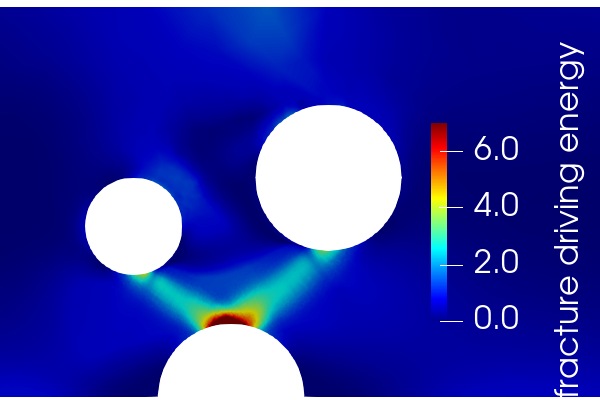
\includegraphics[width=\textwidth,scale=0.5]{prelim/figures/model_1_total_1.png}
        \caption{}
    \end{subfigure}
    \hspace{0.05\textwidth}
    \begin{subfigure}{0.23\textwidth}
        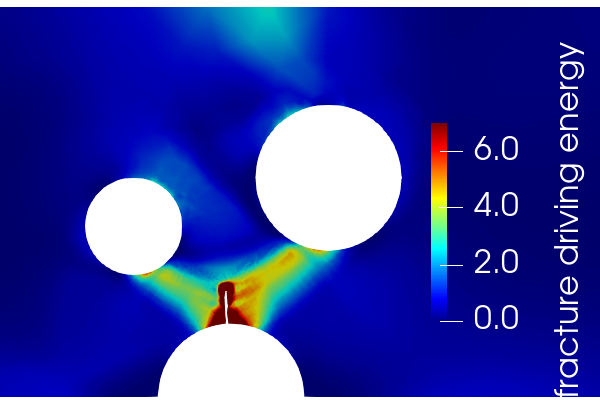
\includegraphics[width=\textwidth,scale=0.5]{prelim/figures/model_1_total_2.png}
        \caption{}
    \end{subfigure}
    \hspace{0.05\textwidth}
    \begin{subfigure}{0.23\textwidth}
        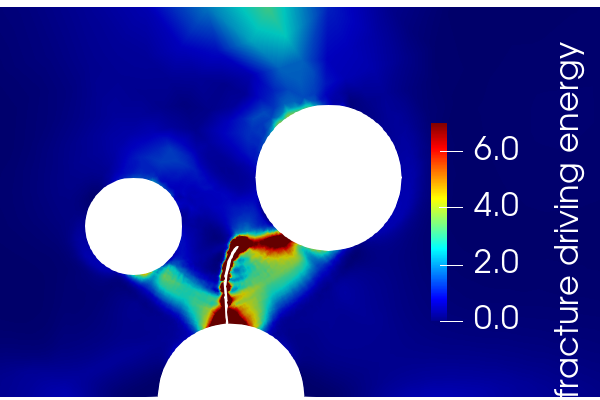
\includegraphics[width=\textwidth,scale=0.5]{prelim/figures/model_1_total_3.png}
        \caption{}
    \end{subfigure}

    \begin{subfigure}{0.23\textwidth}
        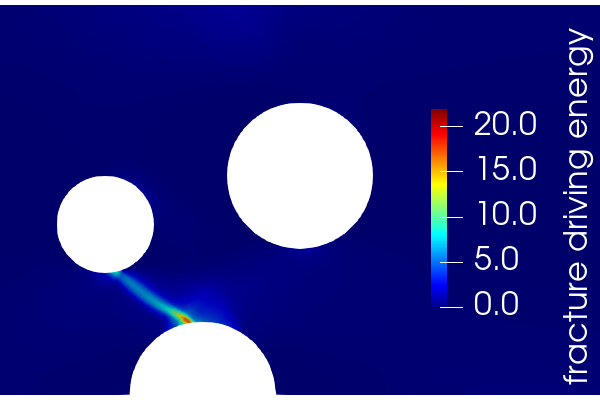
\includegraphics[width=\textwidth,scale=0.5]{prelim/figures/model_2_total_1.png}
        \caption{}
    \end{subfigure}
    \hspace{0.05\textwidth}
    \begin{subfigure}{0.23\textwidth}
        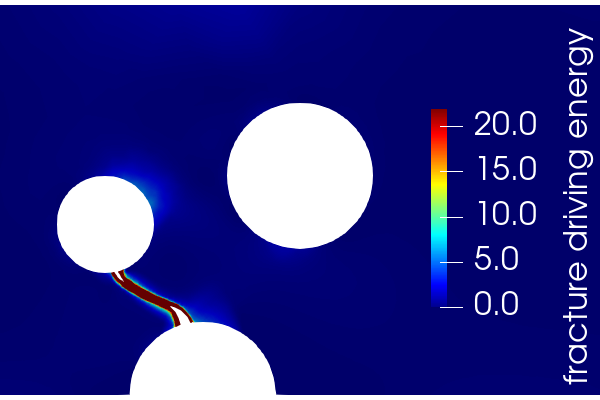
\includegraphics[width=\textwidth,scale=0.5]{prelim/figures/model_2_total_2.png}
        \caption{}
    \end{subfigure}
    \hspace{0.05\textwidth}
    \begin{subfigure}{0.23\textwidth}
        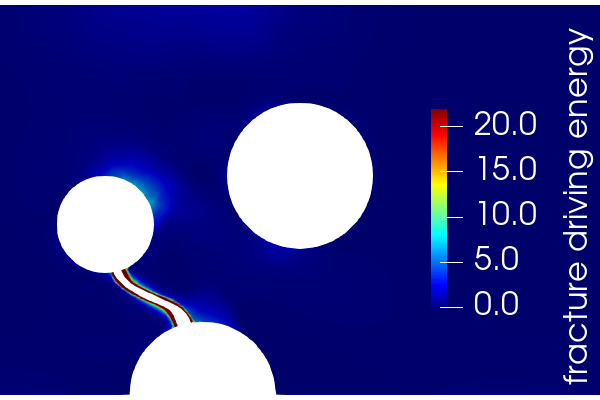
\includegraphics[width=\textwidth,scale=0.5]{prelim/figures/model_2_total_3.png}
        \caption{}
    \end{subfigure}
    \caption{ Contour plots of the total fracture driving energy $\pi_\elastic^\activeenergy + \pi_\plastic$ for (a-c) Dugdale's cohesive model and (d-f) Barenblatt's cohesive model. }
\end{figure}

\end{frame}
